\documentclass[border=10pt]{standalone}
\usepackage{tikz}
\usetikzlibrary{arrows.meta,calc}
\definecolor{cwork}{RGB}{46,137,205}
\definecolor{crepair}{RGB}{235,55,45}
\definecolor{cpm}{RGB}{255,140,0}
\begin{document}
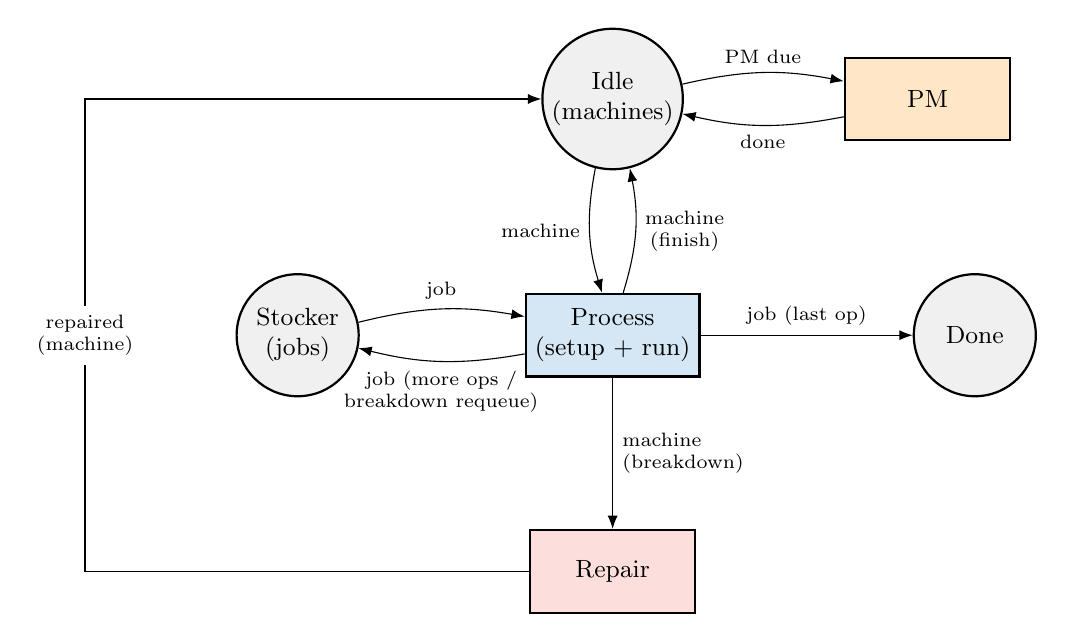
\begin{tikzpicture}[font=\small,>=Latex,
   q/.style={circle,draw,thick,fill=gray!12,minimum size=1.55cm,align=center,inner sep=1pt},
   a/.style={draw,thick,minimum width=2.1cm,minimum height=1.05cm,align=center}]
  % queues (circles = waiting/idle states)
  \node[q] (st)   at (0,0)   {Stocker\\(jobs)};
  \node[q] (idle) at (4,3)   {Idle\\(machines)};
  \node[q] (done) at (8.6,0) {Done};
  % activities (rectangles)
  \node[a,fill=cwork!20]   (proc) at (4,0)  {Process\\(setup + run)};
  \node[a,fill=crepair!16] (rep)  at (4,-3) {Repair};
  \node[a,fill=cpm!22]     (pm)   at (8,3)  {PM};
  % --- job flow ---
  \draw[->] (st) to[bend left=12] node[above,font=\scriptsize]{job} (proc);
  \draw[->] (proc) to[bend left=12] node[below,font=\scriptsize,align=center]{job (more ops /\\ breakdown requeue)} (st);
  \draw[->] (proc) -- (done) node[midway,above,font=\scriptsize]{job (last op)};
  % --- machine flow ---
  \draw[->] (idle) to[bend right=14] node[left,font=\scriptsize]{machine} (proc);
  \draw[->] (proc) to[bend right=14] node[right,font=\scriptsize,align=center]{machine\\(finish)} (idle);
  \draw[->] (proc) -- (rep) node[midway,right,font=\scriptsize,align=left]{machine\\(breakdown)};
  \draw[->] (rep.west) -- (-2.7,-3) -- (-2.7,3) -- (idle.west);
  \node[font=\scriptsize,align=center,fill=white] at (-2.7,0) {repaired\\(machine)};
  \draw[->] (idle) to[bend left=12] node[above,font=\scriptsize]{PM due} (pm);
  \draw[->] (pm) to[bend left=12] node[below,font=\scriptsize]{done} (idle);
\end{tikzpicture}
\end{document}
